\documentclass[aspectratio=169]{beamer}
\usetheme{simple}
\usepackage[english]{babel}
\usepackage[utf8]{inputenc} 
\usepackage{lmodern}
\usepackage{ragged2e}
\usefonttheme[onlymath]{serif} 
\usepackage[scale=2]{ccicons} 
% \setbeamertemplate{caption}[numbered]
\usepackage{copyrightbox}

\usepackage{graphicx,hyperref,url,pgfplots}
\usepackage{amsmath} 
\usepackage{array,booktabs}
\pgfplotsset{compat=1.13}
\usepackage{bibentry}
\usepackage[alf,abnt-etal-list=0,abnt-etal-cite=2]{abntex2cite}
\usepackage[normalem]{ulem}

\usepackage[
    type={CC},
    modifier={by-nc-sa},
    version={4.0},
]{doclicense}

\setbeamercovered{invisible} 
% \newcommand{\pausar}{\pause}
\newcommand{\pausar}{\pause}
\newcommand{\df}[1]{\,\mathrm{d}#1}
\newcommand{\parcial}[3]{\dfrac{\partial^{#1}#2}{\partial #3^{#1}}}
\newcommand{\cpright}[2]{\copyrightbox[b]{#1}{\tiny Source: #2}}

\usepackage{tikz}
\usetikzlibrary{automata,positioning}
\usepackage{xcolor} 
\usetikzlibrary{scopes}
\usepackage{verbatim}
\usetikzlibrary{patterns}

\usepackage{listings}
  \lstdefinestyle{ascii-tree}{
    literate={├}{|}1 {─}{--}1 {└}{+}1 
  }
	\definecolor{codegreen}{rgb}{0,0.6,0}
	\definecolor{codegray}{rgb}{0.5,0.5,0.5}
	\definecolor{codepurple}{rgb}{0.58,0,0.82}
	\definecolor{backcolour}{rgb}{0.92,0.92,0.92}
	\lstset{language=Python, 
	backgroundcolor=\color{backcolour},   
	commentstyle=\color{codegreen},
	keywordstyle=\color{magenta},
	numberstyle=\tiny\color{codegray},
	stringstyle=\color{codepurple},
	basicstyle=\fontsize{8}{11}\ttfamily,
	frame=lines,
%	numbers=left, 
	tabsize=2,
	morekeywords={models, lambda, forms},
	showstringspaces=false}

\usepackage{catchfile}
\newcommand{\getenv}[2][]{%
	\CatchFileEdef{\temp}{"|kpsewhich --var-value #2"}{\endlinechar=-1}%
	\if\relax\detokenize{#1}\relax\temp\else\let#1\temp\fi}

\getenv[\BIBREF]{RM_REFERENCES} 

% --------------------------------------------------------------------------------------------

\title{Mobile Robots}
\subtitle{ROS - Robot Operating System}
\date{\today}
\author[Jeferson José de Lima]{
  \textbf{Professor}: Jeferson José de Lima}
\institute{Academic Department of Informatics (DAINF) \\ Federal University of Technology - Paraná (UTFPR) at Pato Branco, PR, Brazil}

\begin{document}
\maketitle
\justify

\begin{frame}{Useful Information}

	\begin{block}{License}
        \doclicenseThis
    \end{block}
 
	\begin{block}{links:}
		\begin{enumerate}
			\item \href{}{Moodle}
			\item \href{https://gitlab.com/cursoseaulas/robotica-movel/-/wikis/home}{Mobile Robots - Gitlab Page}
			\item \href{http://www.rsl.ethz.ch/education-students/lectures/ros.html}{ETH Programming for Robotics - ROS}
		\end{enumerate}
	\end{block}
\end{frame}

\begin{frame}{What is ROS?}
	\framesubtitle{ROS - Robot Operating System}
	\centering
	
\includegraphics[width=0.4\textwidth]{./images/roslogo.png}
	\begin{block}{About ROS}
		The Robot Operating System (ROS) is a flexible framework for writing robot software. It is a collection of tools, libraries, and conventions that aim to simplify the task of creating complex and robust robot behavior across a wide variety of robotic platforms \cite{noauthor_ros.org_nodate}.

		{\tiny \textbf{More info}: 
		https://www.ros.org/about-ros/}
	\end{block}
\end{frame}


\begin{frame}{History of ROS}
	\framesubtitle{}
	\begin{itemize}
		\item Originally developed in 2007 at the Stanford Artificial Intelligence Laboratory;
		\item Since 2013 managed by Open Source Robotics Foundation, Inc. (OSRF);
		\item Today used by many robots, universities and companies\footnote[frame]{\textcolor{purple}{ https://rosindustrial.org/about/description }};
		\item De facto standard for robot programming;
	\end{itemize}
\end{frame} 

\begin{frame}{ROS Philosophy}
	\framesubtitle{}
	\begin{itemize}
		
		\item \textbf{Peer to peer}: Individual programs communicate over defined API (ROS messages, services, etc.).
		\item \textbf{Distributed}: Programs can be run on multiple computers and communicate over the network.
		\item \textbf{Multi-lingual}: ROS modules can be written in any language for which a client library exists (C++, Python, Julia, MATLAB, Java, etc.).
		\item \textbf{Light-weight}: Stand-alone libraries are wrapped around with a thin ROS layer.
		\item \textbf{Free and open-source}: Most ROS software is open-source and free to use.

	\end{itemize}
\end{frame}


\begin{frame}[fragile]{ROS Master}
	\framesubtitle{ }
	\begin{minipage}{0.6\textwidth}
    \begin{itemize}
        \item Manages the communication between nodes (processes)
        \item Every node registers at startup with the master
    \end{itemize}
	
	\vspace{0.3in}

	\begin{itemize}
		\item Start a master with:

		\begin{lstlisting}[language=bash]
	$ roscore
		\end{lstlisting}

		\item \textbf{roscore} will start up a ROS Master, a ROS Parameter Server and a rosout logging node
		
		\begin{lstlisting}[language=bash]
	$ roscore -p $PORT -w $NUM_WORKERS
		\end{lstlisting}
		\end{itemize}

	\end{minipage}
	\begin{minipage}{0.4\textwidth}
		\centering
\resizebox{0.85\textwidth}{!}{
\begin{tikzpicture}[>=stealth,
    auto,
    state/.append style={fill=black!20, circle, draw, minimum size=2.2cm},
    node distance=1.2cm,
    every text node part/.style={align=center}] 
    \node[state, fill=red!35] (MASTER) {\textbf{ROS} \\ \textbf{Master}};
    \node[state,below right=of MASTER] (SENSOR) {\textbf{Sensor} \\ \textbf{Node}};
    \node[state,below left=of MASTER] (LISTENER) {\textbf{Listener} \\ \textbf{ Sensor} \\ \textbf{Node}};
    \draw (LISTENER) edge[->,bend left=15] node[left] {Subscribe \\ Registration} (MASTER);
    \draw (SENSOR) edge[->,bend right=15] node[right] {Publish \\ Registration} (MASTER);
    \draw (LISTENER) edge[-, dashed] node[blue] {\textbf{/sensor/value}} node[below, red] {std\_msg/Float64} (SENSOR);

\end{tikzpicture}}

	\end{minipage}
\end{frame}

\begin{frame}[fragile]{ROS Nodes}
	\framesubtitle{ }
	\begin{minipage}{0.6\textwidth}
    \begin{itemize}
        \item Single-purpose, executable program;
        \item Individually compiled, executed, and managed;
        \item Organized in \textcolor{purple}{packages};
    \end{itemize}

	Run a \textbf{node} with:
	\begin{lstlisting}[language=bash]
		$ rosrun package_name node_name
    \end{lstlisting}

	See active \textbf{nodes} with:
	\begin{lstlisting}[language=bash]
		$ rosnode list
    \end{lstlisting}

	Retrieve information about a \textbf{node} with
	\begin{lstlisting}[language=bash]
		$ rosnode info node_name
    \end{lstlisting}


\end{minipage}
\begin{minipage}{0.4\textwidth}
	\centering
\resizebox{0.85\textwidth}{!}{
\begin{tikzpicture}[>=stealth,
    auto,
    state/.append style={fill=black!20, circle, draw, minimum size=2.2cm},
    node distance=1.2cm,
    every text node part/.style={align=center}] 
    \node[state, fill=red!35] (MASTER) {\textbf{ROS} \\ \textbf{Master}};
    \node[state,below right=of MASTER] (SENSOR) {\textbf{Sensor} \\ \textbf{Node}};
    \node[state,below left=of MASTER] (LISTENER) {\textbf{Listener} \\ \textbf{ Sensor} \\ \textbf{Node}};
    \draw (LISTENER) edge[->,bend left=15] node[left] {Subscribe \\ Registration} (MASTER);
    \draw (SENSOR) edge[->,bend right=15] node[right] {Publish \\ Registration} (MASTER);
    \draw (LISTENER) edge[-, dashed] node[blue] {\textbf{/sensor/value}} node[below, red] {std\_msg/Float64} (SENSOR);

\end{tikzpicture}}

\end{minipage}
\end{frame}

\begin{frame}[fragile]{ROS Topics}
	\framesubtitle{ }
	\begin{minipage}{0.6\textwidth}
    \begin{itemize}
        \item Nodes communicate over topics;
        \begin{itemize}
			\item Nodes can publish or subscribe to a topic;
			\item Typically, 1 publisher and n subscribers;
		\end{itemize}
        \item Topic is a name for a stream of messages;
        \item Third item
    \end{itemize}
	List active topics with:
	\begin{lstlisting}[language=bash]
		$ rostopic list
    \end{lstlisting}
	Subscribe (CLI) and print the contents of a topic with:
	\begin{lstlisting}[language=bash]
		$ rostopic list
    \end{lstlisting}
	Show information about a topic with:
	\begin{lstlisting}[language=bash]
		$ rostopic echo /topic_name
    \end{lstlisting}
\end{minipage}
\begin{minipage}{0.4\textwidth}
	\centering
\resizebox{0.85\textwidth}{!}{
\begin{tikzpicture}[>=stealth,
    auto,
    state/.append style={fill=black!20, circle, draw, minimum size=2.2cm},
    node distance=1.2cm,
    every text node part/.style={align=center}] 
    \node[state, fill=red!35] (MASTER) {\textbf{ROS} \\ \textbf{Master}};
    \node[state,below right=of MASTER] (SENSOR) {\textbf{Sensor} \\ \textbf{Node}};
    \node[state,below left=of MASTER] (LISTENER) {\textbf{Listener} \\ \textbf{ Sensor} \\ \textbf{Node}};
    \draw (LISTENER) edge[->,bend left=15] node[left] {Subscribe \\ Registration} (MASTER);
    \draw (SENSOR) edge[->,bend right=15] node[right] {Publish \\ Registration} (MASTER);
    \draw (LISTENER) edge[-, dashed] node[blue] {\textbf{/sensor/value}} node[below, red] {std\_msg/Float64} (SENSOR);

\end{tikzpicture}}

\end{minipage}
\end{frame}

\begin{frame}[fragile]{ROS Messages}
	\framesubtitle{ }
	\begin{minipage}{0.6\textwidth}
    \begin{itemize}
        \item Data structure defining the type of a topic
		\item Comprised of a nested structure of integers, floats, booleans, strings etc. and arrays of objects
		\item Defined in *.msg files
		\begin{lstlisting}[language=bash]
	$ rosmsg list
		\end{lstlisting}
		\item you can type rosmsg to look up its fields:
		\begin{lstlisting}[language=bash]
	$ rosmsg info PROJECT_NAME/MESSAGE_NAME
	...
		\end{lstlisting}

		\item An example:
		\begin{lstlisting}[language=bash]
	$ rosmsg info ros_examples/Sensor 
	string name
	float32 temperature
	float32 humidity	
		\end{lstlisting}

    \end{itemize}

\end{minipage}
\begin{minipage}{0.4\textwidth}
	\centering
\resizebox{0.85\textwidth}{!}{
\begin{tikzpicture}[>=stealth,
    auto,
    state/.append style={fill=black!20, circle, draw, minimum size=2.2cm},
    node distance=1.2cm,
    every text node part/.style={align=center}] 
    \node[state, fill=red!35] (MASTER) {\textbf{ROS} \\ \textbf{Master}};
    \node[state,below right=of MASTER] (SENSOR) {\textbf{Sensor} \\ \textbf{Node}};
    \node[state,below left=of MASTER] (LISTENER) {\textbf{Listener} \\ \textbf{ Sensor} \\ \textbf{Node}};
    \draw (LISTENER) edge[->,bend left=15] node[left] {Subscribe \\ Registration} (MASTER);
    \draw (SENSOR) edge[->,bend right=15] node[right] {Publish \\ Registration} (MASTER);
    \draw (LISTENER) edge[-, dashed] node[blue] {\textbf{/sensor/value}} node[below, red] {std\_msg/Float64} (SENSOR);

\end{tikzpicture}}

\end{minipage}
\end{frame}


\begin{frame}[fragile]{catkin Build System}
	\framesubtitle{ }
    \begin{itemize}
        \item The \textbf{catkin} workspace contains the following spaces

		\begin{lstlisting}[style=ascii-tree]
		~/catkin_ws $ tree -L 1
		├── build				<-------- do not touch
		├── devel				<-------- do not touch
		└── src					<-------- work here
			├── turtlebot3
			├── YOUR_PACKAGE
			└── ...
		\end{lstlisting}

		\item \textbf{/src}: \textcolor{blue}{The source space contains the source code. This is where you can clone, create, and edit source code for the packages you want to build}
		\item \textbf{/build}: \textcolor{red}{The build space is where CMake is invoked to build the packages in the source space. Cache information and other intermediate files are kept here.}
		\item \textbf{/devel}: \textcolor{red}{The development (devel) space is where built targets are placed (prior to being installed)}
		\end{itemize}
\end{frame}


\begin{frame}[fragile]{Creating a ROS Package}
	\framesubtitle{ }
    \begin{itemize}
        \item First of all, you need to change to the source space directory of the catkin workspace
		\begin{lstlisting}[language=bash]
	$ cd ~/catkin_ws/src
		\end{lstlisting}
		\item catkin\_create\_pkg requires that you give it a package\_name and optionally a list of dependencies on which that package depends:
		\begin{lstlisting}[language=bash]
	$ catkin_create_pkg <package_name> [depend1] [depend2] [depend3]
		\end{lstlisting}
		\item This is an example:
		\begin{lstlisting}[language=bash]
			$ catkin_create_pkg beginner_tutorials std_msgs rospy roscpp
		\end{lstlisting}

	\end{itemize}
\end{frame}

\begin{frame}[fragile]{ROS Messages}
	\framesubtitle{ }
	\begin{minipage}{0.6\textwidth}
    \begin{itemize}
        \item Data structure defining the type of a topic
		\item Comprised of a nested structure of integers, floats, booleans, strings etc. and arrays of objects
		\item Defined in *.msg files
		\begin{lstlisting}[language=bash]
	$ rosmsg list
		\end{lstlisting}
		\item you can type rosmsg to look up its fields:
		\begin{lstlisting}[language=bash]
	$ rosmsg info PROJECT_NAME/MESSAGE_NAME
	...
		\end{lstlisting}

		\item An example:
		\begin{lstlisting}[language=bash]
	$ rosmsg info ros_examples/Sensor 
	string name
	float32 temperature
	float32 humidity	
		\end{lstlisting}

    \end{itemize}

\end{minipage}
\begin{minipage}{0.4\textwidth}
	\centering
\resizebox{0.85\textwidth}{!}{
\begin{tikzpicture}[>=stealth,
    auto,
    state/.append style={fill=black!20, circle, draw, minimum size=2.2cm},
    node distance=1.2cm,
    every text node part/.style={align=center}] 
    \node[state, fill=red!35] (MASTER) {\textbf{ROS} \\ \textbf{Master}};
    \node[state,below right=of MASTER] (SENSOR) {\textbf{Sensor} \\ \textbf{Node}};
    \node[state,below left=of MASTER] (LISTENER) {\textbf{Listener} \\ \textbf{ Sensor} \\ \textbf{Node}};
    \draw (LISTENER) edge[->,bend left=15] node[left] {Subscribe \\ Registration} (MASTER);
    \draw (SENSOR) edge[->,bend right=15] node[right] {Publish \\ Registration} (MASTER);
    \draw (LISTENER) edge[-, dashed] node[blue] {\textbf{/sensor/value}} node[below, red] {std\_msg/Float64} (SENSOR);

\end{tikzpicture}}

\end{minipage}
\end{frame}

\begin{frame}[t,fragile]{ROS Exercice}
	\framesubtitle{\textcolor{purple}{Create a Temperature Sensor Node. Use your favorite language C++ or Python}}
	\begin{minipage}{0.6\textwidth}
		\begin{itemize}
			\item \textcolor{blue}{\textbf{Example - Sensor Node (Python)}}:
		\end{itemize}
	\begin{lstlisting}
	import rospy
	from std_msgs.msg import Int32

	def sensor():
		pub = rospy.Publisher('sensor/value', 
								Int32, queue_size=10)
		rospy.init_node('sensor_node',
						anonymous=False)
		rate = rospy.Rate(1) # Hz
		i = 0
		while not rospy.is_shutdown():
			sensor_msg = "value %s" % i
			rospy.loginfo(sensor_msg)
			pub.publish(i)
			rate.sleep()
			i = i + 1
			...
    \end{lstlisting}
\end{minipage}
\begin{minipage}{0.4\textwidth}
	\centering
\resizebox{0.85\textwidth}{!}{
\begin{tikzpicture}[>=stealth,
    auto,
    state/.append style={fill=black!20, circle, draw, minimum size=2.2cm},
    node distance=1.2cm,
    every text node part/.style={align=center}] 
    \node[state, fill=red!35] (MASTER) {\textbf{ROS} \\ \textbf{Master}};
    \node[state,below right=of MASTER] (SENSOR) {\textbf{Sensor} \\ \textbf{Node}};
    \node[state,below left=of MASTER] (LISTENER) {\textbf{Listener} \\ \textbf{ Sensor} \\ \textbf{Node}};
    \draw (LISTENER) edge[->,bend left=15] node[left] {Subscribe \\ Registration} (MASTER);
    \draw (SENSOR) edge[->,bend right=15] node[right] {Publish \\ Registration} (MASTER);
    \draw (LISTENER) edge[-, dashed] node[blue] {\textbf{/sensor/value}} node[below, red] {std\_msg/Float64} (SENSOR);

\end{tikzpicture}}

\end{minipage}
\end{frame}


\begin{frame}[fragile]{ROS Exercice}
	\framesubtitle{\textcolor{purple}{Create a Temperature Sensor Node. Use your favorite language C++ or Python}}
	\begin{minipage}{0.6\textwidth}
	\begin{itemize}
		\item \textcolor{blue}{\textbf{Example - Sensor Node (Python)}}:
	\end{itemize}
	\begin{lstlisting}[language=Python]
		...
		if __name__ == '__main__':
		try:
			sensor()
		except rospy.ROSInterruptException:
			pass
	
    \end{lstlisting}
	\begin{block}{Remember, you need to give execute permission to the ROS:}
		Type this command in the Terminal:
		\begin{lstlisting}[language=Python]
		$ chmod +x sensor_node.py
		\end{lstlisting}
	\end{block}
\end{minipage}
\begin{minipage}{0.4\textwidth}
	\centering
\resizebox{0.85\textwidth}{!}{
\begin{tikzpicture}[>=stealth,
    auto,
    state/.append style={fill=black!20, circle, draw, minimum size=2.2cm},
    node distance=1.2cm,
    every text node part/.style={align=center}] 
    \node[state, fill=red!35] (MASTER) {\textbf{ROS} \\ \textbf{Master}};
    \node[state,below right=of MASTER] (SENSOR) {\textbf{Sensor} \\ \textbf{Node}};
    \node[state,below left=of MASTER] (LISTENER) {\textbf{Listener} \\ \textbf{ Sensor} \\ \textbf{Node}};
    \draw (LISTENER) edge[->,bend left=15] node[left] {Subscribe \\ Registration} (MASTER);
    \draw (SENSOR) edge[->,bend right=15] node[right] {Publish \\ Registration} (MASTER);
    \draw (LISTENER) edge[-, dashed] node[blue] {\textbf{/sensor/value}} node[below, red] {std\_msg/Float64} (SENSOR);

\end{tikzpicture}}

\end{minipage}
\end{frame}


\begin{frame}[fragile]{ROS Exercice}
	\framesubtitle{\textcolor{purple}{Create a Temperature Sensor Node. Use your favorite language C++ or Python}}
	\begin{minipage}{0.6\textwidth}
	\begin{itemize}
		\item \textcolor{blue}{\textbf{Example - Listener Node (C++)}}:
	\end{itemize}
	\begin{lstlisting}[language=C++]
#include "ros/ros.h"
#include "std_msgs/Int32.h"

void callback(const std_msgs::Int32::ConstPtr& msg)
{
	ROS_INFO("I heard: %d", msg->data);
}

int main(int argc, char **argv)
{
	ros::init(argc, argv, "listener");
	ros::NodeHandle n;
	ros::Subscriber sub=n.subscribe("/sensor/value", 
							1000, callback);
	ros::spin();
	return 0;
}
	
    \end{lstlisting}
\end{minipage}
\begin{minipage}{0.4\textwidth}
	\centering
\resizebox{0.85\textwidth}{!}{
\begin{tikzpicture}[>=stealth,
    auto,
    state/.append style={fill=black!20, circle, draw, minimum size=2.2cm},
    node distance=1.2cm,
    every text node part/.style={align=center}] 
    \node[state, fill=red!35] (MASTER) {\textbf{ROS} \\ \textbf{Master}};
    \node[state,below right=of MASTER] (SENSOR) {\textbf{Sensor} \\ \textbf{Node}};
    \node[state,below left=of MASTER] (LISTENER) {\textbf{Listener} \\ \textbf{ Sensor} \\ \textbf{Node}};
    \draw (LISTENER) edge[->,bend left=15] node[left] {Subscribe \\ Registration} (MASTER);
    \draw (SENSOR) edge[->,bend right=15] node[right] {Publish \\ Registration} (MASTER);
    \draw (LISTENER) edge[-, dashed] node[blue] {\textbf{/sensor/value}} node[below, red] {std\_msg/Float64} (SENSOR);

\end{tikzpicture}}

\end{minipage}
\end{frame}


\begin{frame}{ROS Exercice}
	\framesubtitle{\textcolor{purple}{Create a Temperature Sensor Node. Use your favorite language C++ or Python}}
	Result:
	\begin{figure}
		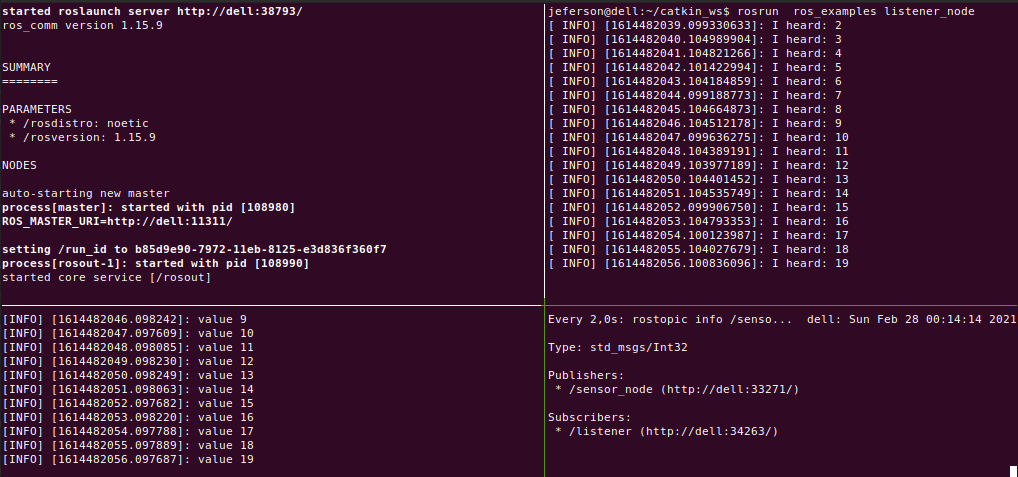
\includegraphics[width=1\textwidth]{./images/ros_sensor_example.png}
	\end{figure}
\end{frame}


\begin{frame}[fragile]{ROS Messages}
	\framesubtitle{Creating a ROS msg}
    \begin{itemize}
        \item Let's define a new msg in the package. Save the MyMessage.msg file in \$PROJECT\_NAME/msg:
		\begin{lstlisting}[language=bash]
	$ echo "string name
	> int32 temperature" > msg/MyMessage.msg
		\end{lstlisting}
		\item Open package.xml, and make sure these two lines are in it and uncommented:
		\begin{lstlisting}[language=bash]
	<build_depend>message_generation</build_depend>
	<exec_depend>message_runtime</exec_depend>
		\end{lstlisting}
		\item Add the message\_generation dependency to the find\_package call which already exists in your CMakeLists.txt so that you can generate messages
		\begin{lstlisting}[language=bash]
	find_package(catkin REQUIRED COMPONENTS
		roscpp
		rospy
		std_msgs
		message_generation
	)
		\end{lstlisting}

	
    \end{itemize}
% \footnote[frame]{\textbf{More info}: \href{http://wiki.ros.org/ROS/Tutorials/CreatingMsgAndSrv}{ROS/Tutorials/CreatingMsgAndSrv}}
\end{frame}

\begin{frame}[fragile]{ROS Messages}
	\framesubtitle{Creating a ROS msg\footnote[frame]{\textcolor{purple}{\textbf{More info}: \href{http://wiki.ros.org/ROS/Tutorials/CreatingMsgAndSrv}{ROS/Tutorials/CreatingMsgAndSrv}}}}
    \begin{itemize}
        \item Uncomment it by removing the \# symbols and then replace for MyMessage.msg:
		\begin{lstlisting}[language=bash]
		add_message_files(
			FILES
			MyMessage.msg
			)
		\end{lstlisting}
		\item For ROS Hydro and later, you need to uncomment these lines:
		\begin{lstlisting}[language=bash]
	# generate_messages(
		#   DEPENDENCIES
		#   std_msgs
		# )
		\end{lstlisting}
		\item Compile and test it:
		\begin{lstlisting}[language=bash]
		$ cd ~/catkin_ws && catkin_make
		$ python -c "from PROJECT_NAME.msg import MyMessage; print(MyMessage)"
		\end{lstlisting}
    \end{itemize}

\end{frame}



\begin{frame}{ROS}
	\framesubtitle{But ...}
	\centering
	\begin{block}{Projects are becoming more complex ... }
		\begin{figure}
			\cpright{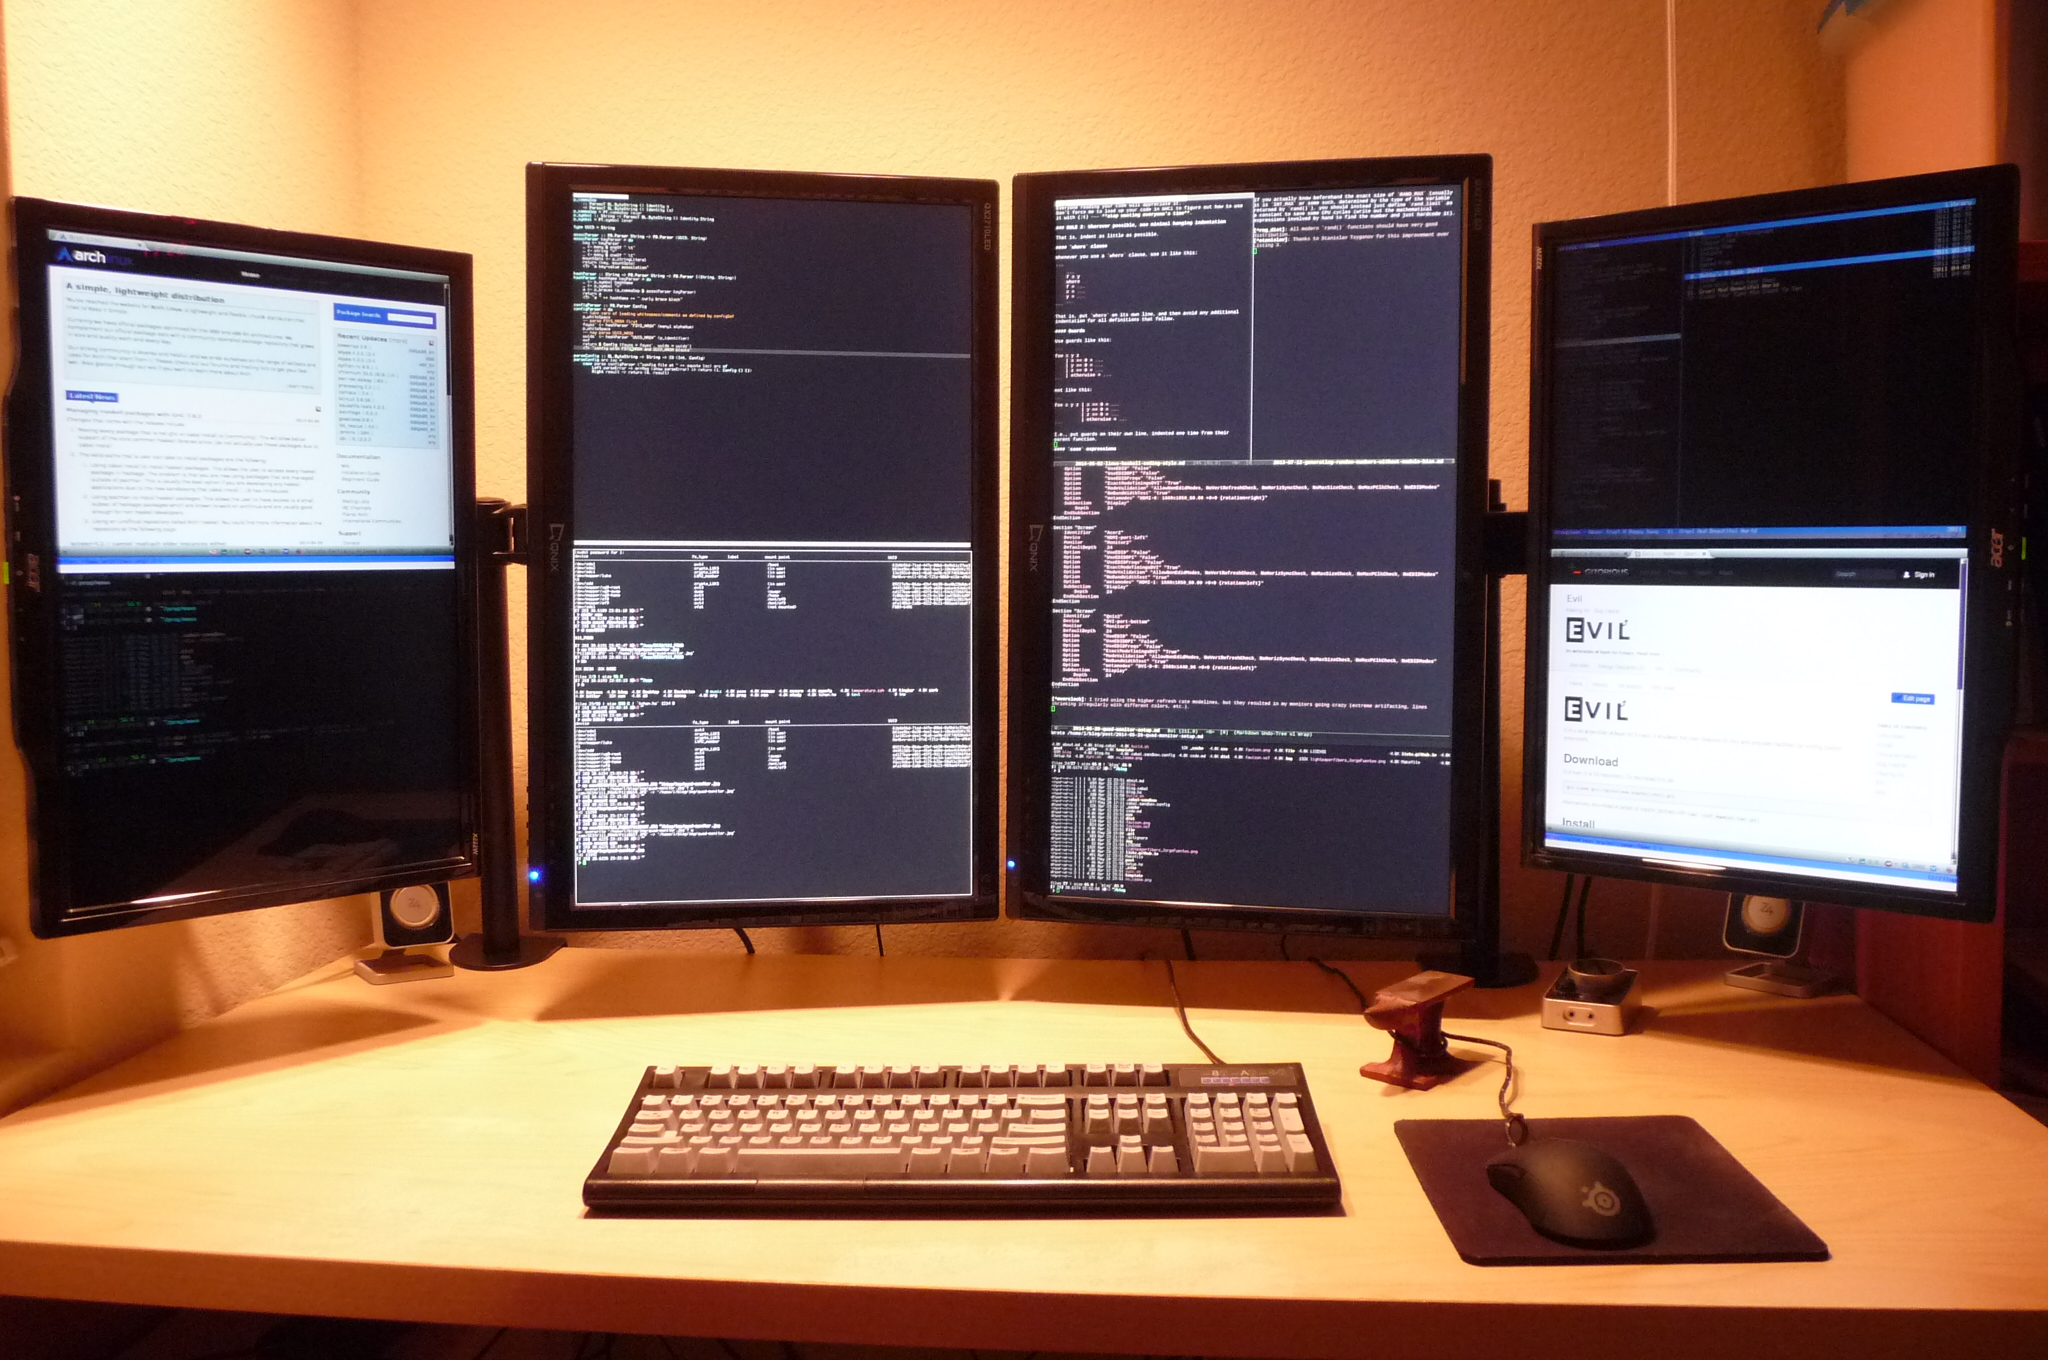
\includegraphics[width=0.6\textwidth]{./images/rossetup.jpg}}
			{https://www.theproductexaminer.com/monitors/best-monitor-setup-for-programming.html}
		\end{figure}
	\end{block}
\end{frame}


\begin{frame}[fragile]{ROS Launch}
	\framesubtitle{Evaluates the XML file in a single pass}
	\begin{itemize}
		\item \textit{launch} is a tool for launching multiple nodes (as well as setting parameters)
		\item Are written in XML as \textit{*.launch} files
		\item If not yet running, launch automatically starts a roscore
	\end{itemize}

	Browse to the folder and start a launch file with:
	
	\begin{lstlisting}[language=bash]
		$ roslaunch file_name.launch
	\end{lstlisting}

	Start a launch file from a package with

	\begin{lstlisting}[language=bash]
		$ roslaunch roslaunch package_name file_name.launch
	\end{lstlisting}
\end{frame}


\begin{frame}[fragile]{ROS Launch}
	\framesubtitle{Evaluates the XML file in a single pass}
	\begin{itemize}
		\item \textit{launch} is a tool for launching multiple nodes (as well as setting parameters)
		\item Are written in XML as \textit{*.launch} files
		\item If not yet running, launch automatically starts a roscore
	\end{itemize}

	Browse to the folder and start a launch file with:
	
	\begin{lstlisting}[language=bash]
		$ roslaunch file_name.launch
	\end{lstlisting}

	Start a launch file from a package with

	\begin{lstlisting}[language=bash]
		$ roslaunch package_name file_name.launch
	\end{lstlisting}
\end{frame}



\begin{frame}[fragile]{ROS Launch}
	\framesubtitle{}

	\begin{itemize}
		\item This basic sample shows \textit{roslaunch} runtime:
	
	\begin{block}{roslaunch my\_project turtlesim\_and\_teleop.launch}
		\begin{lstlisting}[language=XML]
	<?xml version="1.0" ?>
	<launch>
		<node pkg="turtlesim" name="turtlesim_simulador" type="turtlesim_node"></node>
		<node pkg="turtlesim" name="turtlesim_control"  type="turtle_teleop_key"></node>
	</launch>
		\end{lstlisting}
	\end{block}

		\item \textbf{launch:} Root element of the launch file;
		\item \textbf{node:} Each node tag specifies a node to be launched;
		\item \textbf{name:} Name of the node (free to choose);
		\item \textbf{pkg:} Package containing the node;
		\item \textbf{type:} Type of the node, there must be a corresponding executable with the same name;
		\item \textbf{output:} Specifies where to output log messages (screen: console, log: log file);
	
	\end{itemize}

\end{frame}

\begin{frame}[t, allowframebreaks]
	\frametitle{Referências}
	\bibliography{\BIBREF}
\end{frame}

\end{document}